\section{The lattice}\label{sec:lbm:lattice}
symmetry... multi speed... weights ... D2Q9

\begin{equation}\label{eq:lbm:weights}
w_i = 
\left\{
  \begin{array}{l l}
    4/9 & \quad \text{if $i = 0$}\\ 
    1/9 & \quad \text{if $i = 1,2,3,4$}\\    
    1/36 & \quad \text{if $i = 5,6,7,8$}\\
  \end{array} \right.
\end{equation}

\begin{equation}\label{eq:lbm:d2q9_c}
\{\ci\} = \left\{
\begin{bmatrix}0\\0\end{bmatrix}, 
\begin{bmatrix}1\\0\end{bmatrix}, 
\begin{bmatrix}0\\1\end{bmatrix}, 
\begin{bmatrix}-1\\0\end{bmatrix}, 
\begin{bmatrix}0\\-1\end{bmatrix}, 
\begin{bmatrix}1\\1\end{bmatrix}, 
\begin{bmatrix}-1\\1\end{bmatrix}, 
\begin{bmatrix}-1\\-1\end{bmatrix}, 
\begin{bmatrix}1\\-1\end{bmatrix}
\right\} 
\end{equation}

\begin{figure}
  \centering
  \subfloat[D2Q7
    ]{\label{fig:lbm:h1}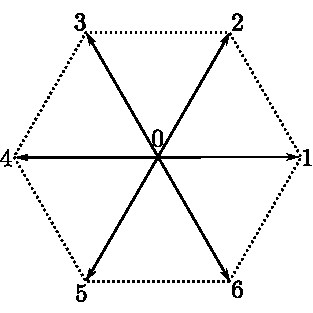
\includegraphics[width=0.47\textwidth]{fig/lattice_d2q7.pdf}}      
  \hspace{5pt}
  \subfloat[D2Q9
    ]{\label{fig:lbm:h2}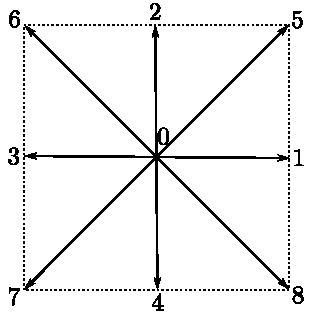
\includegraphics[width=0.45\textwidth]{fig/lattice_d2q9.pdf}} 
  \caption{Two different unit cells for lattices used in the LBM in two
    dimensions. In (a) the D2Q7 seven speed lattice is shown and in
    (b) the nine speed D2Q9 lattice. The numbering at the edges is the
    usual naming convention for the different velocities.}
  \label{fig:lbm:lattices}
\end{figure}
